\section{Actividad 6}

Armar Fig.~\ref{fig:3} en GNU Radio.  

\begin{figure}[h!]
    \centering
    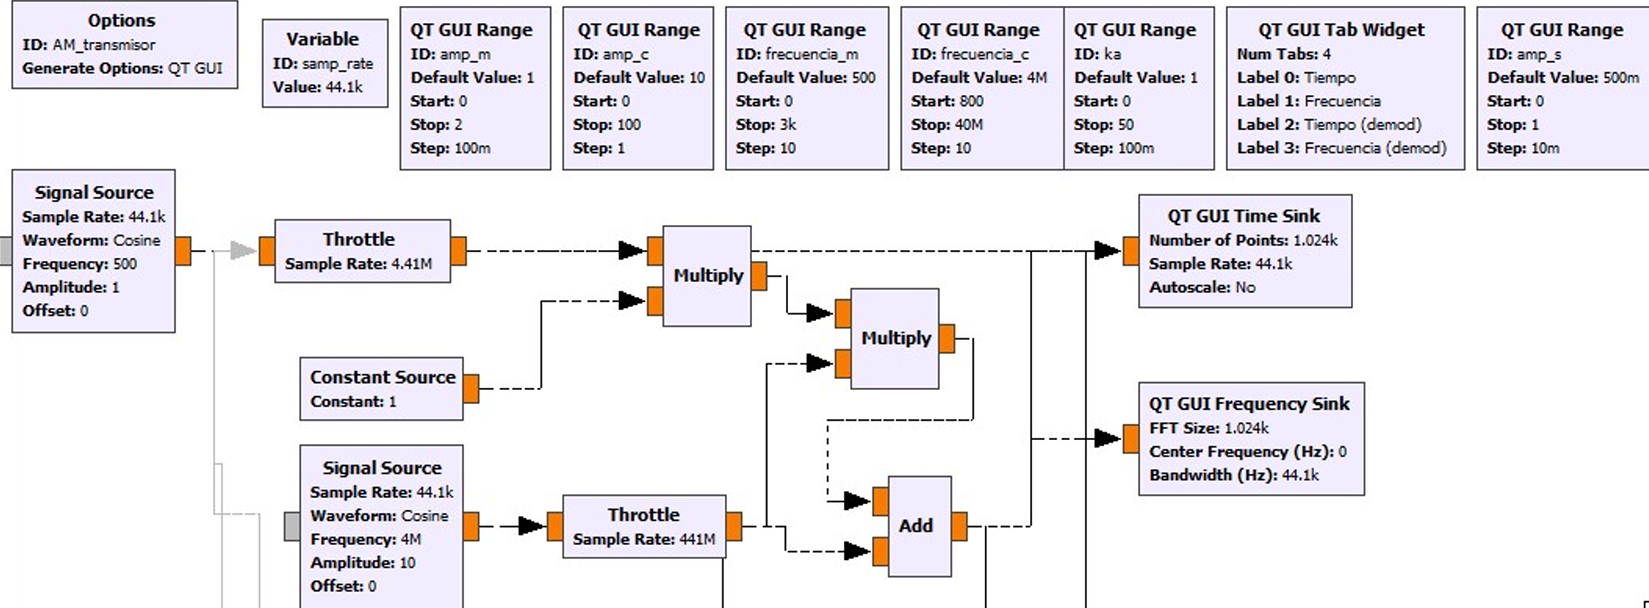
\includegraphics[width=0.6\textwidth]{fig3.png}
    \caption{Esquema en GNU Radio}
    \label{fig:3}
\end{figure}

\begin{itemize}
    \item[a)] ¿Qué es GNU Radio?  
    \item[b)] ¿Qué es SDR?  
    \item[c)] Expresar $s(t)$.  
    \item[d)] Explicar bloques de la Fig.~\ref{fig:3}.  
    \item[e)] Graficar señales para 10\%, 60\% y 100\%.  
    \item[f)] Graficar sobre-modulación.  
    \item[g)] Analizar espectro en cada caso.  
    \item[h)] Implementar receptor y recuperar señal.  
\end{itemize}